\begin{exercises}

\exercise 在卡文迪许实验中(参考图\ref{fig:04.04}),设$ M $与$  $m的中心都在同一
圆周上,两个大球分别处于同一直径之两端,各与近处小球之球心
距为$  r = 1 0 . 0   $厘米,轻杆长$  l = 5 0 . 0  $ 厘米, $ M = 1 0 . 0  $千克,$  m = 1 0 . 0  $
克,悬杆的角偏转$  \theta = 3 . 9 6 \times 1 0 ^ { - 8 }  $弧度,悬丝的扭转常数$  k = 8 . 3 4
  \times 1 0 ^ { - 8 }  $千克$ \cdot $米$ ^2 $/秒$ ^2 $。试求$ G $之值。

\exercise 试计算太阳对月球的引力$ F _ {\text{日}\to\text{月}} $以及地球对月亮的引力
$ F _ {\text{月}\to\text{日}} $,并比较二者的大小。

\exercise 已知地球中心与月球中心相距$  s = 3 . 8 4 \times 1 0 ^ 5 $公里,地球质
量$ M _ {\text{地}} $与月球质量$ M _ {\text{月}}$之比为$ 81:1 $。有一星际飞船从地球飞向月
球,船中乘客在通过地球引力区和月球引力区的分界线时,没有
测到重力,试求此处距地球多远?

\exercise 有一根无限长的直线,线密度为$ \rho $。试问:与它相距为$ x $处
% 151.jpg
的一个质量为$ M $的质点所受的引力等于多少?方向指向哪里?

\exercise 有一根质量为$ M $、长为$ 2L $的直线。将坐标系原点取在直
线的中点,直线为$ y $轴,过中点的垂线取为$ x $轴。

(1)有一质量为$  m _ { 1 }   $的质点在$  P _ { 1 } \left( x, 0 \right)   $位置,求这直线作用于
$  m _ { 1 }   $上的引力表达式及引力的方向;

(2)有一质量为$  m _ { 2 }   $的质点在$  P _ { 2 } \left( 0, y \right)   $位置,求这直线作用于
$  m _ { 2 }   $上的引力表达式及引力的方向;

(3)如果$  L = 1   $米,线密度$  \rho = 2  $克/厘米, $ m _ { 2 } = 0 . 5   $克,$ y = 3  $ 米,
试问:$ 2L $作用于$  m _ { 2 }   $上的引力之值是多少?

\exercise 如果太阳的质量突然减少一半,试问地球轨道(假定是圆)
会发生什么变化?

\exercise 设某一星系中的体为均匀球状分布,该星系的总质量为
$ M $,半径为$  R _ { 0 } $。距星系心为$  r < R _ { 0 }   $处有一质量为$ M _ 1 $的星体,
$ M _ 1 $在引力作用下作圆周运动。问:

(1)$  M _  1    $所受的引力是多少?

(2)$ M _ 1 $作同周运动的率是多少?

\exercise 已知月球的质量约为地球质量的$ 1/81 $,其直径约为地球
直径的3/11,若不计由于地、月自转引起的重量变化。试问:在
地球上重60公斤的人,在月球上用弹簧秤称得的体重是多少?

\exercise 已知火星的平均直径为6900公里,地球的平均直径为$ 1.3
  \times 1 0 ^ { 4 }   $公里,火星质量约为地球质量$  M _ { E }   $的0.11倍。试求:

(1)火星的平均密度$\rho$与地球的平均密度$ \rho _ E $之比;

(2)火星表面的$ g $值。

\exercise 试由月球绕地球运行的周期($  T = 2 7 . 3   $天)和轨道半径
($  r = 3 . 8 5 \times 1 0 ^ { 5 } $ 公里)(设为圆轨道),来确定地球的质量$ M _ e $。

\exercise 地球绕太阳公转周期$  T \approx 3 6 5   $日,地日距离$  r \approx 1 . 4 9 \times 1 0 ^ { 8 }  $
公里,设地球轨道为圆形,求太阳质量$ M _ \text{日} $。

\exercise 已知太阳离银心距离约为$  2 . 4 \times 1 0 ^ { 2 0 }   $米,太阳绕银心转一
% 152.jpg
周约需$  2 . 5 \times 1 0 ^ { 8 }   $年。设大阳运行轨道为圆形,银河系中恒星的平
均质量与太阳相等。试估计银河系中太阳轨道以内的恒星个数。

\exercise 在一个质量为$ M $,半径为$ R $的铅球中挖一个半径为$ R/2 $的
空腔,使它的表面与铅球球面相切。在铅球中心与空腔中心的连
线上,且离铅球中心距离为$ d $处放一个质量为$ m $的小球(图\ref{fig:04.12})。
试求在这种情况下铅球与小球之间的引力$ \vec{F} $。
\begin{figurex}
  \centering
  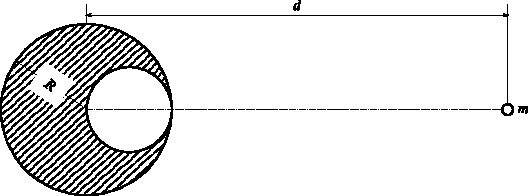
\includegraphics{figure/fig04.12}
  \caption{}
  \label{fig:04.12}
\end{figurex}

\exercise 有一密度均匀的球壳,外半径为$ a $,内半径为$ b $,总质量为
$ M $。在离球心$ r $处有一质量为$ m $的质点,$ r $的范围为$  0 \leqslant r \leqslant \infty   $。试
筒略地画出球壳对$ m $的引力$ F $与$ r $之间的函数曲线。

\exercise 一人造地球卫星以圆形轨道环绕地球飞行,其周期为$  T =
  90.0 $分钟。已知地球半径为$  R = 6. 3 7 \times 1 0 ^ { 3 }   $公里,质量为$  M _ { E } = 5 . 9 8
  \times 1 0 ^ { 2 7 }   $克,万有引力常数为$  G = 6 . 6 7 \times 1 0 ^ { - }  8 $厘米\.$ ^3 $/克$ \cdot $\.$ ^2 $。求卫星离
地面的高度$ h $。

\exercise 同步卫星广泛用于地球范围内的电视转播和通讯。它在
地球上空以地球自转的角速度绕地心转动,这就使它能停留在地
面某一确定点的上空。求:

(1)同步卫星的轨道相对地球的方位;

(2)同步卫星轨道的半径有多大?

\exercise 关于中子星问题:

(1)有一密度均匀的球体,以角频率$ \omega $围绕自身的几何对称
% 153.jpg
轴旋转。若维持其表面物质不因快速旋转被甩掉的力只有引力,这
球体的密度$ \rho $至少要多大?

(2)蟹状星云(经过认证,它是我国北宋至和元年,即公元
1054年观测到的一次超新星爆发的遗迹)中有一颗脉冲星,它每秒
转30周。以此数据估算这颗脉冲星的最小密度。

(3)若此脉冲星的质量约为一个太阳的质量$ M _ \text{日} $(约$  2 \times 1 0 ^ { 3 0 }  $
公斤或约$  3 \times 1 0 ^ { 5 } M _ { E }  $)  ,试问:它的最小的可能半径是多少?

\exercise 在地面上重16公斤的物体,在以$  a = g / 2 $ ($ g $为地面处的重
力加速度)上升的人造地球卫星里,视重为9.0公斤。这时该卫星
离地面多远?

\exercise 一密度均匀的球形天体,半径为$ R $,它的质量$ M $至少为
多大时,才会使它的第一宇宙速度大于光在真空中的速度?

\exercise 一密度均匀的球形天体,它的质量等于太阳质量$ M _ \text{日} =
  1. 9 8 \times 1 0 ^ { 3 0 }  $公斤,问它的半径$ R $最大为多少时,才会使它的第一宇宙速度大于光在真空中的速度?

\exercise 一行星沿椭圆轨道绕大阳运行,离大阳最近时(距离为$ r $)
速度最大,记为$ V $;离太阳最远时(距离为$ R $)速度最小,记为$ v $。

(1)证明$ \dfrac { V } { v } = \dfrac { R } { r }   $。

(2)地球绕太阳公转,在远日点的速度为29.2公里/秒。已知
地球轨道的偏心率为0.01674,求地球在近日点公转的速度。

\exercise 设某行星绕中心天体在圆轨道上运行,公转周期为$ T $。用
开普勒第三定律证明:一个物体从此轨道由静止自由落至中心天
体所需的时间为$d = \dfrac { T } { 4 \sqrt { 2 } } $。

\exercise (1)一物体在月球轨道上,设只受地球引力,由静止开始
自由落向地球。不计地球大气的阻力,求落到地面所需的时间t和
落地时的速度$ v $。
% 154.jpg

(2)一物体在地球轨道上,设只受太阳引力,由静止开始自
由落向太阳,不计阻力,求落到太阳表面所需的时间和到达太阳
表面时的速度。

\exercise 哈雷彗星绕日运动的周期为76年,估计它的远日点到太
阳的距离。

\end{exercises}